\documentclass[12pt]{article}
\usepackage{report}

%\usepackage[acronym]{glossaries}
\usepackage{rotating}
\usepackage{float}
\usepackage{physics}
\usepackage{siunitx}
\usepackage{array}
\usepackage[justification=centering]{caption}
%\captionsetup[figure]{font=small
\usepackage{booktabs}
\usepackage[table,xcdraw]{xcolor}
\usepackage{chngcntr}
\usepackage[utf8]{inputenc}
\usepackage{listings}
%\usepackage{subfigure}
\usepackage{subcaption}
\usepackage{tocloft}
\usepackage{indentfirst}
\usepackage{enumitem}
%\usepackage[acronym,nomain]{glossaries}
% \usepackage{pracalik}
\usepackage{acronym}
%\makeglossaries
\usepackage[square,numbers]{natbib}
\bibliographystyle{ieeetr}
%\bibliographystyle{abbrvnat}
%\usepackage[sectionbib]{natbib}
%\usepackage{chapterbib}
%\usepackage{biblatex} %Imports biblatex package
%\bibliographystyle{ieeetr}
%\addbibresource{biblio.bib}

%\renewcommand{cfttoctitlefont}{12pt}
\setcounter{secnumdepth}{3} % for subheadings
\setlength{\cfttabindent}{0pt} %for tables
\setlength{\cftfigindent}{0pt} %for figures


\title{Tr-Level Segmented CNN }
\author{ GROUP 04 }
\date{\today}



\begin{document}


\thispagestyle{empty} % This will hide pagenumber in title page

% Title page (Design in your own way)

% First title page
\begin{titlepage}
\begin{center}
        \textit{A Minor Project Report\\}
        \textit{on\\}
		\begin{LARGE}
		\bf{Detection of Brain tumor using Convolutional neural networks with transfer learning\\}
		\end{LARGE}
		\vspace{20pt}
		\textit{submitted in partial fulfillment of the requirements for the award of degree\\}
		\vspace{10pt}
		\textbf{\Large Bachelor of Technology\\}
		\vspace{4pt}
		\text{in}\\
		\vspace{4pt}
		\textbf{\Large Computer Science and Engineering}\\
		\vspace{10pt}
		
		{\bf by} \\[1.0cm]
 
 \begin{table}[h!]
\begin{center}
\begin{tabular}{c c} 
 \textbf{\Large 21211A05X7} & \textbf{\Large Vattikuti Harini sri ramya}\\[0.5ex] 
 \textbf{\Large 21211A05Y2} & \textbf{\Large Sai Kaushik}\\[0.5ex]
 \textbf{\Large 21211A05V4} & \textbf{\Large Syed Arif}\\[0.5ex]
 \textbf{\Large 22215A05W0} & \textbf{\Large Vijay Kumar}
\end{tabular}
\end{center}
\end{table} 
		\vspace{10pt}
		
\includegraphics[width=0.3\textwidth]{img/logo.jpg} \\
		\vspace{8pt}
		\textit{Under the kind guidance of}\\
		\textbf{\large S Anjanayya}\\
		
		\vspace{8pt}
		
		{\bf Laboratory:} Data Science\\
		\textbf{\Large{Department of Computer Science and Engineering}\\
			\Large{B V Raju Institute of Technology}\\
   \vspace{4pt}  
             \small{(UGC Autonomous, Accrediated by NBA and NAAC)\\
             Vishnupur,Narsapur, Medak(Dist), Telangana State, India-502313.}\\
}
	\end{center}

\end{titlepage}



\pagenumbering{roman} % roman page numbers


\section*{\Large\centering \textbf{CERTIFICATE OF APPROVAL}}
\addcontentsline{toc}{section}{CERTIFICATE OF APPROVAL}

This project work (Batch ID) entitled " {\bf Detection of brain tumor using Convolutional neural netwoeks with transfer learning} " by Mr. Your Name, Registration No. 123456789 under the supervision of Mr. Supervisor in the Department of Computer Science and Engineering, B V Raju Institute of Technology, Narsapur, is hereby submitted for the partial fulfillment of completing Minor Project during II B.Tech    II Semester (2022 - 2023 EVEN). This report has been accepted by Research Domain Computer vision and forwarded to the Controller of Examination, B V Raju Institute of Technology, also submitted to Department Special Lab " Data Science"  for the further procedures.\\
\\
\\

\noindent
\begin{tabular}{l}
$\overline{\text{{\bf S Anjanayya}}}$ \\
{\bf Associate Professor and Supervisor}\\
Department of CSE\\
B V Raju Institute of Technology\\
Narsapur.\\
\\
\\
\\
\\
$\overline{\text{{\bf External Examiner}}}$ \\
\end{tabular}
\hfill % move it to the right
\begin{tabular}{l}
$\overline{\text{{\bf Dr.CH.Madhu Babu}}}$ \\
{\bf Professor and Dept.Head}\\
Department of CSE\\
B V Raju Institute of Technology\\
Narsapur\\
\\
\\
\\
\\
$\overline{\text{{\bf Internal Examiner}}}$ \\
\end{tabular}
\\
\\
\\
\\
\\
{\centering
\begin{tabular}{l}
$\overline{\text{{\bf Dr.D.vivek}}}$ \\
\bf Lab Incharge - Data Science\\
Department of Computer Science and Engineering\\
B V Raju Institute of Technology\\
Narsapur
\end{tabular}\par}
\newpage


%% Put declaration, letter of approval and copyright only in the final report

\newpage
\section*{DECLARATION} 
\addcontentsline{toc}{section}{DECLARATION}
%\setcounter{page}{1} 
\vspace{1mm}
\quad We, the members of Research Group domain \textbf{computer vision} under \textbf{Data Science } special lab , declare that this report titled: \textbf{Detection of brain tumor by convolutional neural network by transfer learning } is our original work and has been submitted in whole or in parts for International conference or journal \textbf{Knowledge Management, Artificial Intelligence, and Telecommunication Engineering (RMKMATE)}. All sources of information used in this report have been acknowledged and referenced respectively.

\quad This project was undertaken as a requirement for the completion of our \textbf{II B.Tech II Sem Minor project} in Department of \textbf{Computer Science and Engineering} at \textbf{B V Raju Institute of Technology}, Narsapur. The project was carried out between 31-March-2023 and 11-August-2023. During this time, we as a team were responsible for the process model selection, development of the micro document and designing of the project.

\quad  Detection of brain tumor using cnn by transfer learning is plays an key role in detection of tumor in accurate and effective way. this project leads to identifying the tumor in accurate way by using vgg16.

\quad We would like to express our gratitude to our project supervisor Dr.D.vivek for his guidance and support throughout this project. We would also like to thank our Department Head Dr.CH.Madhu babu for his help and efforts. We also thank the Dental experts for providing valuable insights into a mandible anotomy, which greatly assisted in the development of segmentation model.

\quad We declare that this report represents Our own work, and any assistance received from others has been acknowledged and appropriately referenced.







\vskip 1mm
  {\bf}
Vattikuti Harini sri ramya\hspace{1.3cm}(21211A05X7) \hspace{0.4cm}  \rule{0.3\textwidth}{0.5pt}
\vskip 0.1mm
Sai Kaushik\hspace{2.1cm}(21211A05Y2) \hspace{0.4cm}  \rule{0.3\textwidth}{0.5pt}
\vskip 0.1mm
Syed Arif\hspace{2.1cm}(21211A05V4) \hspace{0.4cm}  \rule{0.3\textwidth}{1pt}
\vskip 0.1mm
Vijay Kumar\hspace{2.0cm}(22215A05W0) \hspace{0.4cm}  \rule{0.3\textwidth}{1pt}
\vspace{0.3cm} 


\textbf{Supervisor}\hspace{1.5cm}\textbf{Project Coordinator}\hspace{1.5cm}\textbf{Dr.D.Vivek}\hspace{1.5cm}\textbf{HOD/CSE}





%% This is constant for all the reports 
% Acknowledgments
\newpage
\section*{ACKNOWLEDGEMENT}
\addcontentsline{toc}{section}{ACKNOWLEDGEMENT}
\quad This project is prepared in fulfilment of the requirement for the \textbf{Data  Science  Lab} under Research Domain \textbf{Computer  Vision}. We owe our deepest gratitude to the Department of Computer Science and Engineering \break B V Raju Institute of Technology, Narsapur for providing us with an opportunity to work on this project.
\vspace{0.2cm}

\quad We also extend our gratitude towards our project supervisor \textbf{Dr.D.Vivek} and Department Head \textbf{Dr.Madhu babu} , whose guidance and expertise have been invaluable in steering us towards success. We also thank other faculty members of the Department for their valuable feedback and suggestions.

\quad Finally, we would like to thank our family and friends for their continuous support and encouragement throughout the project. We acknowledge the contributions of everyone who supported us in the creation of this project report.

\quad Thank you all for your assistance and support.


\quad The experience of working on this project will surely enrich our
technical knowledge and also give us hands on experience of working on a project and help develop our team's skill set to a great extent.




\newpage
\section*{\Large\centering \textbf{ABSTRACT}}
\addcontentsline{toc}{section}{ABSTRACT}
This review of the literature examines the
application of transfer learning methods and convolutional neural
networks (CNNs) for the identification of brain tumours, especially using the VGG16 architecture. Brain tumours are a serious
health issue, and detecting them early is essential to enhancing patient outcomes. In applications involving medical image
analysis, such as tumour diagnosis, CNNs have demonstrated
considerable potential. Transfer learning enables maximising the
performance of the target task by exploiting the information
obtained from pre-trained models. With a focus on the VGG16
model, we examine and evaluate pertinent literature in this survey
that discusses the application of CNNs and transfer learning for
brain tumour identification. The survey’s results shed light on the
cutting-edge techniques, difficulties, and potential future paths in this area\\
\hfill \vspace{1cm} \break 
\small
\noindent \textbf{\textit{Keywords:}} CNN, tumor, brain x-ray images,vgg16.








\newpage

\newpage
\addcontentsline{toc}{section}{LIST OF FIGURES}
\listoffigures





\newpage

\newpage
\addcontentsline{toc}{section}{LIST OF TABLES}
\listoftables





\newpage

\newpage
\section*{\Large\centering \textbf{LIST OF ACRONYMS AND ABBREVIATIONS}}
\addcontentsline{toc}{section}{LIST OF ACRONYMS AND ABBREVIATIONS}



 
% Acronym definitions
\begin{acronym}
\acro{VGG16}{ Visual Geometry Group}
\acro{CNN}{ convolutional neural network}
\acro{TL}{Transfer learning}

  
\end{acronym}

 
%\Print the glossary

%\printglossary[type=\acronymtype]
%\printglossaries





\newpage

% Table of contents

\newpage
{
  \setlength{\parskip}{0em}
  \renewcommand\contentsname{TABLE OF CONTENTS} % This will change heading text
  \tableofcontents %\addcontentsline{toc}{section}{TABLE OF CONTENTS}
}



% List of Abbreviation- if any

\newpage

\newpage
\pagenumbering{arabic}
\begin{center}
    \textbf{\LARGE CHAPTER - 1}
\end{center}

\section{INTRODUCTION}

 Brain is an important organ of our body.Brain plays an key role in transfering the information and used to makes the key activities.So diseases causes due to brain leads to danger and so curation in an important ,so we should cure them and identify them is an important.we will explore how the brain tumor is detected in an accurate way by using vgg16.  CNN with transfer learning makes the detection easy and accurate with high effectient way.
% \clearpage
\vspace{0.25cm}
\subsection{Background}

 Convolutional Neural Networks (CNNs): CNNs are a class of deep learning models specifically designed for image recognition and classification tasks. They have revolutionized computer vision and are widely used in medical image analysis, including brain tumor detection.
Transfer Learning: Transfer learning is a technique where a pre-trained neural network, such as VGG16, is used as a starting point for a new task. Instead of training a network from scratch, you fine-tune the pre-trained model's weights on your specific dataset. This is particularly useful when you have limited data for your target task.
VGG16 Architecture: VGG16 is a popular deep learning architecture known for its simplicity and effectiveness. It consists of 16 layers (13 convolutional and 3 fully connected) and is particularly good at capturing fine-grained features in images. \cite{einstein}.



\vspace{0.25cm}
\subsection{Motivation} 

Medical Impact: Brain tumors are a serious and life-threatening medical condition. Developing a reliable and accurate tool for early detection can potentially save lives and improve the quality of life for patients. Knowing that your work can contribute to advancements in medical science is highly motivating.
Humanitarian Aspect: Brain tumor detection can be a critical aspect of healthcare, especially given the devastating consequences of late-stage diagnoses. Contributing to the field of healthcare can be deeply rewarding on a personal level.
working on a project to detect brain tumors using CNN with transfer learning, such as VGG16, offers a compelling blend of technical challenges, personal fulfillment, and the opportunity to make a meaningful impact on healthcare and society. It can be a highly motivating and rewarding endeavor for anyone passionate about both technology and healthcare.
\vspace{0.25cm}

\subsection{Problem statement}

\begin{itemize}
\item   The aim of improving the diagnostic accuracy and reducing the need for invasive procedures.
\item  The goal of this project is to develop CNN with transfer
learning to automate the detection of brain tumors in MRI
scans
\item  this project aims to build a CNN model with transfer
learning to reduce time and error rate in manual interpretation.
\end{itemize}

\subsection{Objectives}


\begin{enumerate}
\item  Use a CNN with transfer learning to identify brain
cancers with excellent accuracy in MRI scans.
\item  Reduce false positive and false negative results in the detection process to maintain the system’s high reliability
and accuracy

\item  Compare the CNN model’s effectiveness with other
current techniques for detecting brain tumours in MRI
images.
\end{enumerate}

\subsection{Scope of Project}

To gain an insight into the scope of our project, let us first understand what the term scope of a project means in software development, the scope refers to the boundaries and limitations of a project. It also defines the features, functions, and requirements of the software being developed. The scope of a software project describes what the software will and will not do, and what is included and excluded from the project. 

Detection of  brain tumor by cnn using transfer learning will consist of two primary functionalities:  

The project aims to deliver the following key features:

\begin{itemize}
    \item  Early Detection: Detect brain tumors at an early stage when intervention and treatment can be more effective, potentially improving patient outcomes.
\vspace{0.5cm}
    \item  Increase the accuracy of brain tumor diagnosis by leveraging the powerful feature extraction capabilities of CNNs and the knowledge learned from a large dataset like ImageNet.
    \item  Reduce the risk of human error in the interpretation of medical images by providing automated assistance to radiologists and clinicians.
\end{itemize}


The boundaries and limitations of detection of brain tumor can also be defined by its scope, which also outlines the features, functions, and requirements of the system. Some of these boundaries and limitations are:

\begin{itemize}
    \item \textbf{Data Quality and Quantity}:  Data quality refers to the accuracy, consistency, and reliability of the dataset used for training and evaluation. In medical image analysis, especially for tasks like brain tumor detection.
     \item \textbf{Hardware and Computational Resources}: Detecting brain tumors using Convolutional Neural Networks (CNNs) with transfer learning, such as VGG16, is a computationally intensive task. The hardware and computational resources required for this task depend on various factors, including the size of your dataset, the complexity of the model, and the level of optimization.
    \item \textbf{Incorporating Clinical Context}:  ncorporating clinical context is crucial when using Convolutional Neural Networks (CNNs) with transfer learning, such as VGG16, for the detection of brain tumors. Clinical context enhances the utility and interpretability of the model's results, making them more valuable for healthcare professionals.
    \item \textbf{Complexity of Brain's  Structures}: Complexity of Brain's Structures.
\end{itemize}


Addressing these limitations through ongoing research, collaboration with brain professionals, and continuous model refinement will be essential for maximizing the model's potential impact on dental diagnostics and treatment planning.
 
Overall, the project report will provide a comprehensive understanding of the detection of Brain structure of  CNN. The report will serve the accuracy and effectiency in detection of brain tumor.
\newpage
%\pagenumbering{arabic}
\begin{center}
    \textbf{\LARGE CHAPTER - 2}
\end{center}
\section{LITERATURE SURVEY}
 The human body is composed of a variety of cell
types. The brain is a delicate and highly specialised organ
of the human body. The benign or malignant form of brain
tumour can be identified. The malignant is cancerous whereas
the benign is not. Malignant tumor is classified into two types:
primary and secondary tumor. Detection of brain tumor is an
one of the challenge for human because of its structure.
Tumors are divided into primary and secondary categories.
Because of its structure, detecting brain tumours is one of the
most difficult tasks for humans.
Brain picture segmentation is necessary for brain tumour
detection. Segmenting MR images of the brain manually is
challenging. It takes a lot of time, is a difficult process
that cannot be repeated, needs non-uniform segmentation, and
segmentation outcomes might differ from expert to expert.
Automated brain tumour segmentation and identification is
fraught with problems. Brain tumour segmentation is a challenging problem for an autonomous computer system since it
requires pathology, MRI physics, as well as intensity and form
analysis of the MRI picture. The main problem in segmenting
brain tumours is that they differ in terms of form, size,
location, and picture intensities. A computer-aided approach
for brain tumour identification and segmentation is preferable
since manual segmentation of brain tumours involves human
specialists and takes a lot of time.
Therefore in this situation, computer assisted system is beneficial. The classification of the brain MR image as normal
or tumorous should be accurate and take less time with an
automated brain tumour detection method. It must be reliable
and provide radiologists an intuitive, user-friendly solution that
is self-explanatory
The most fatal illness, brain tumours have an extremely low
life expectancy in their most severe form. Brain tumour misdiagnosis will lead to ineffective medical treatment and lower
patient survival rates. Developing an appropriate treatment
strategy to treat and prolong the lives of people with brain
tumours depends on making an accurate diagnosis of the
disease.
Using clinical brain scans, Balakumar et al. [2] developed
an automated segmentation of brain tumour identification.
Compared to manual tumour analysis, automatic segmentation
of brain tumours is far superior. In this study, the brain tumour
areas are to be retrieved using region-based segmentation. For
additional processing, the shape, intensity, and texture-based
characteristics need to be extracted. The post processing technique may be used to do the spatial regularisation. The strength
of this research is in its ability to categorise structural elements
into normal and pathological tissue using discriminative traits,
which further reduces complexity. The paper’s flaw is that the
edge-based approach fails when the image is too complicated
or blurry to clearly show a boundary.
A probabilistic neural network-based method for identifying
brain tumours was proposed by Dina Aboul Dahab et al. In this
study, a customised PNN model is built utilising MRI scans
to analyse data and images while learning vector quantization.
At the preprocessing stage, the image’s edges are smoothed
using a Gaussian filter. The color-based segmentation approach
should be utilised in this situation since it produces better
results than the kmeans algorithm. ROI uses a modified version
of the canny edge-based detection technique. The postprocessing stage makes use of the modified PNN algorithm. This
paper’s benefit is that it uses a PNN system based on LVQ,
which lengthens processing time by around 79 percentage of
CNN in PNN.
In recent years, it has been possible to identify brain tumours
in MRI scans using machine learning techniques, most specifically CNN. Yet, the idea of employing MRIs dates to 1984.
For many years, MRI has been a vital imaging tool in the
detection and management of brain malignancies. Manual MRI
interpretation, however, can be laborious, error-prone, and
vulnerable to inter-observer variability. As a result, computeraided diagnosis (CAD) systems have been created to help
radiologists analyse medical pictures.
Convolutional neural networks (CNNs) with transfer learning
have been used to identify brain cancers in MRIs as early
as 2010. Deep learning was becoming more popular at the
time, and scientists were investigating its potential uses in the
processing of medical images. CNN makes it easier to identify
the tumour and takes less time
Havaei et al. carried out one of the first investigations in this
area in 2014. Using T1- weighted contrast-enhanced MRIs,
they classified brain cancers into four groups using a CNN
(glioma, meningioma, pituitary adenoma, and healthy brain
tissue). The network’s accuracy was 90.5being trained on a
dataset of 220 patients.
Another team of University of Michigan researchers
employed transfer learning in 2016 to create a CNN-based
technique for automatically classifying brain tumours in MRI
images. The technique employed a pre-trained CNN model,
which was then refined using a collection of brain MRI
images that had tumour locations labelled. The model was
quite accurate in differentiating between various kinds of
brain cancers. With MRI images, they employed a CNN with
transfer learning to find brain cancers. To extract features from
MRI scans, they employed a pre-trained model (VGG16),
which was initially trained on the ImageNet dataset. They
subsequently improved the model using a dataset of brain
tumour MRIs, and 97 percentage accuracy was attained
\begin{table}[H]
    \centering
    \caption{\small analysis of differents methods.}
   \scriptsize
    \begin{tabular}{lrrrrrrrrrr}
\toprule
{} &  \small Name  &  \small accuarcy   \\

\midrule
1 &    InceptionNet  &    85 percentage   \\
2 &    resNet50  &    89 percentage  \\
3 &    vgg16  &   95 percentage\\

\bottomrule
\end{tabular}
    
    \label{fig:posterior}
\end{table}
\newpage
\pagenumbering{arabic}
\begin{center}
    \textbf {\LARGE CHAPTER - 3}
\end{center}
\section{REQUIREMENT ANALYSIS \& SPECIFICATION}

This section of the project report is the most critical element as, it provides a foundation for the entire project. It ensures that all stakeholders are aligned on the project's objectives, scope, and deliverables, and it provides a clear road map for the project team to follow.\\This section is further divided into 3 sister sections:
\begin{itemize}
    \item Feasibility Study
    \item Model Selection
    \item SRS
\end{itemize}
% \clearpage

\subsection{Feasibility Study}
 A feasibility study is the first stepping stone into the development of any project, including our Tri-
level segmented CNN to predict dental informatics. It involves assessing the potential for the project
to be successful, which in turn includes evaluating the market, technology, financial aspects, and
operational requirements. Conducting a feasibility study on detecting brain tumors in MRIs using a Convolutional Neural Network (CNN) involves assessing the technical, operational, economic, and scheduling aspects of implementing this approach
 
\subsubsection{Market Analysis}
A market analysis involves assessing the current market landscape, potential demand, competition, pricing strategies, and overall market viability. It Provide's an overview of the medical imaging market and the increasing importance of advanced technologies for brain tumor detection and Introduce's the concept of using CNNs with transfer learning for brain tumor detection in MRI images. It Identifies key segments within the market, such as MRI devices, software solutions, and AI-based diagnostic tools
\subsubsection{Technology Assessment}
It involves evaluating the key technologies, tools, advantages, limitations, and future prospects of the approach. It Explain's the fundamentals of CNNs, including their architecture, layers, and operations like convolution, pooling, and fully connected layers. And Describe's how CNNs are particularly well-suited for image processing tasks like medical image analysis. It Discuss the specific ways how  CNNs are utilized in brain tumor detection from MRI images, emphasizing feature extraction and classification
\subsubsection{Operational Requirements}
 Establishing the operational requirements  involves specifying the technical, infrastructure, personnel, and workflow aspects necessary to effectively implement and manage this technology. and Specifies the required computing power, including CPU, GPU, or specialized hardware accelerators, based on the complexity of CNN models and the size of the dataset. It Define's the amount of storage needed for storing MRI datasets, pre-trained models, and intermediate results during training and inference. And also it Determine's the network requirements for transferring large MRI image datasets between storage, preprocessing, training, and inference components.
\subsubsection{Financial Analysis} 
Performing a financial analysis involves assessing the costs associated with developing, deploying, and maintaining the system, as well as potential revenue streams or cost savings generated by its use. Salaries and benefits for data scientists, machine learning engineers, and developers involved in data collection, preprocessing, model selection, training, and integration. And Expenses related are to acquiring, organizing, and preprocessing the MRI data, including any licensing fees, data storage costs, and data augmentation efforts. It Estimate potential revenue or cost savings generated by the brain tumor detection system

\subsubsection{Risk Assessment}
It  involves several risks that should be carefully assessed and managed to ensure the accuracy, safety, and effectiveness of the system. In this the model may be overfit to the training data and perform poorly on unseen data, including misclassifying tumors or generating false positives/negatives. And Implements the  techniques like data augmentation, regularization, and proper model validation to prevent overfitting and enhance model generalization.  The project may exceed the allocated budget due to unforeseen challenges or inadequate cost estimation


\vspace{0.25cm}
\subsection{ Selection of Process Model}
The software life cycle process model is a framework that outlines the various stages involved in the development of a software application. So, choosing a life cycle process model is the stepping stone into the development of a software product.

\subsubsection{ Process Models}
The choice of software development process model for teeth segmentation and future integration of a CNN model for age and gender prediction using GCNN, an iterative and flexible process model would be suitable. One such process model that fits well with AI and deep learning projects is the Agile methodology.

\subsubsection{Why Agile}
Here are some reasons why the Agile model is the best choice for developing teeth segmentation model:

\begin{itemize}
    \item \textbf{Adaptability to Changing Requirements:}  In AI projects, requirements and objectives can evolve rapidly due to advancements in technology or new insights from stakeholders. The Agile model's iterative and incremental approach allows you to adapt to these changes easily, ensuring that your project stays aligned with the latest developments and meets evolving needs.

    \item \textbf{Faster Time-to-Value:} Agile's short development cycles, known as sprints, enable you to deliver working components of the project in a timely manner. This means you can start utilizing and validating the teeth segmentation and AI models early on, providing value to dental professionals and researchers sooner than traditional development approaches.

    \item \textbf{ Continuous Stakeholder Engagement:} Agile emphasizes regular interactions with stakeholders, including dental experts, data scientists, and end-users. This continuous engagement ensures that their feedback and insights are incorporated into the project throughout its lifecycle, resulting in a solution that truly addresses their needs and expectations.
    \item \textbf{Risk Mitigation and Early Issue Identification: } Agile's iterative nature allows for frequent testing and validation of the teeth segmentation and AI models. This early and regular testing helps in identifying potential issues and risks early on in the development process. Addressing these issues promptly minimizes the chances of costly and time-consuming problems later in the project, leading to a more successful and efficient implementation.

\end{itemize}

\subsubsection{Why Not}
Every coin has two sides thus, we can't forget to consider that the waterfall model has some limitations too such as:
\begin{itemize}
    \item Scope Management
    \item Resource Intensive   
\end{itemize}


While Agile offers many benefits, it may not be suitable for projects with fixed, rigid timelines or highly regulated environments, where extensive documentation and upfront planning are mandatory. In such cases, adopting Agile might require careful planning and adaptation to address the specific needs and constraints of the project.













\newpage

\vspace{0.25cm}


\subsection{Software Requirements Specification}
\subsection{Introduction}
\subsubsection{Purpose}
The purpose of detecting brain tumors in MRI images using convolutional neural networks (CNNs) with transfer learning is to improve the accuracy and efficiency of tumor identification. By leveraging pre-trained CNN models, we can harness the knowledge learned from large datasets to enhance the detection of subtle tumor features, aiding in early diagnosis and treatment planning. This approach reduces the need for manual analysis, speeds up the diagnostic process, and ultimately contributes to better patient outcomes in the field of medical imaging.

\subsubsection{Scope}
The Detection of brain tumor with transfer
learning will include the following functionalities:
\begin{itemize}
    \item Enhanced Accuracy: CNNs with transfer learning can provide high accuracy in detecting brain tumors. They can learn relevant features from MRI scans, helping in the differentiation of tumor regions from normal brain tissue. This can aid radiologists in making more accurate and timely diagnoses.
    \item Automation and Efficiency: By automating the initial tumor detection process, CNNs can help radiologists in their workflow, allowing them to focus on more complex tasks and reducing the risk of human error.
\end{itemize}

\subsubsection{Definitions, Acronyms and Abbreviations}
\begin{itemize}
    \item \textbf{Definitions:}\\
    CNN: Convolutional Neural Network\\
    AI: Artificial Intelligence\\
    GCNN: Graph Convolutional Neural Network\\
    SRS: Software Requirements Specification\\
    
    \item \textbf{Acronyms:}\\
    X-ray: Radiograph used in dental imaging\\
    ROI: Region of Interest\\
    FCN: Fully Convolutional Network\\
    IoU: Intersection over Union\\
    GUI: Graphical User Interface\\
    
    \item \textbf{Abbreviations:}\\
    CNN: Convolutional Neural Network\\
    AI: Artificial Intelligence\\
    GCNN: Graph Convolutional Neural Network\\
    SRS: Software Requirements Specification\\
\end{itemize}


\subsubsection{References}
IEEE Std 830-1998, IEEE Recommended Practice for Software Requirements Specifications.

\subsubsection{Overview}
The document will mostly consist of two parts: 
\begin{itemize}
    \item Overall Description
    \item Specific Requirements 
\end{itemize}
Overall description describes the major components of the system, assumptions and dependencies of the system, while specific requirements describes the functions of the system and their roles in the system and the constraints faced by the system.

\subsection{Overall Description}
\subsubsection{Product Perspective}
The product perspective for detecting brain tumors in MRI scans using convolutional neural networks with transfer learning involves implementing advanced machine learning techniques to enhance the accuracy and efficiency of tumor detection. This innovative solution aims to streamline the diagnostic process, providing faster and more reliable results for medical professionals. It leverages pre-trained models to extract meaningful features from MRI images, reducing the need for extensive data annotation and improving generalization. Additionally, the system should offer user-friendly interfaces for radiologists and healthcare practitioners, facilitating seamless integration into clinical workflows. 

\subsubsection{Product Functions}
The key features of the system include:

MRI image upload and processing.
Brain tumor detection using a pre-trained CNN.
User registration and authentication.
User-friendly web interface.


\subsubsection{User Characteristics}
\begin{itemize}
\item \textbf {Radiologists:} These are the primary users who will upload MRI images and review the diagnostic reports.
\item \textbf {Administrators:} Responsible for system maintenance and user management.
\end{itemize}
\subsubsection{Constraints}
The following constraints are considered for the development of the model:
\begin{itemize}
    \item \textbf{Data Availability:} Limited access to diverse and high-quality MRI datasets for brain tumor detection can constrain the effectiveness of convolutional neural networks (CNNs) with transfer learning, as model performance heavily depends on the quantity and diversity of training data.
    \item \textbf{Computational Resources:} Training and fine-tuning CNNs with transfer learning on MRI data often require substantial computational resources, including powerful GPUs and memory, which can be a constraint in resource-limited healthcare settings.
\end{itemize}

\subsubsection{Assumptions \& Dependencies}
The Detecting of brain tumor in MRI’s using a
convolutional neural networks with transfer
learning assumes the following:
\begin{itemize}
    \item  Availability of a sufficient and diverse dataset of MRI brain images containing both tumor and non-tumor cases is essential for training the convolutional neural network (CNN) with transfer learning.
    \item Availability of GPU-accelerated hardware or cloud computing resources is necessary to efficiently train and deploy the CNN
    \item Access to pre-trained CNN models and libraries  for transfer learning is dependent on open-source.
\end{itemize}

\subsection{Specific Requirements}
\subsubsection{External Interfaces}
The Detecting of brain tumor in MRI’s using a
convolutional neural networks with transfer
learning may include the following external interfaces:
\begin{itemize}
    \item Input Data Interface: The system should accept MRI image data as input. These images should adhere to specific formats (e.g., DICOM) commonly used in medical imaging.
    \item User User Interface: If the system is designed for use by medical professionals, create a user-friendly web-based interface or application that allows users to upload MRI images, initiate the detection process, and view the results.
\end{itemize}

\subsubsection{Functions}
The primary functions of the Detecting of brain tumor in MRI’s using a convolutional neural networks with transfer
learning are:
\begin{itemize}
    \item \textbf {Data Preprocessing and Augmentation:}
    \item Data Collection:  Gather a labeled dataset of MRI images with corresponding labels indicating the presence or absence of brain tumors.
    \item Data Preprocessing:  Preprocess the MRI images to enhance features, standardize dimensions, and normalize pixel values.  
    \item \textbf{2.   Transfer Learning:}
    \item Import Pre-trained CNN Model:  Choose a pre-trained CNN model (e.g., VGG16, ResNet, Inception) that was trained on a large dataset (e.g., ImageNet) and remove the final classification layers.
    \item Feature Extraction:  Use the pre-trained CNN to extract features from the MRI images. Freeze the pre-trained layers to retain the learned features.             \item \textbf{Modification and Fine-tuning:}
    \item Add Additional Layers:  Add new layers (fully connected, softmax) on top of the pre-trained CNN to tailor the model for the specific brain tumor detection task.
    \item Fine-tuning:  Unfreeze some of the pre-trained layers and fine-tune the model on the brain tumor dataset to adapt to the specific features relevant to tumor detection.             
    \item \textbf{Compile and Train the Model:}
    \item Compile the Model:  Define the loss function, optimizer, and evaluation metrics (e.g., categorical cross-entropy, Adam optimizer, accuracy).
    \item Train the Model:  Train the modified model using the augmented and preprocessed MRI dataset. Monitor training progress and adjust hyperparameters as needed.            \item \textbf{Model Evaluation and Validation:}
    \item Evaluate the Model:  Assess the model's performance on a separate validation dataset, using metrics like accuracy, precision, recall, F1-score, and confusion matrix analysis.
    \item Fine-tune Further:  Based on evaluation results, fine-tune the model further, adjusting hyperparameters or modifying the architecture to improve performance.      \item \textbf {Inference and Prediction:}
    \item Make Predictions:  Use the trained model to predict brain tumor presence or absence in new MRI images.
    \item Post-processing:  Apply post-processing techniques (e.g., thresholding, morphological operations) to refine predictions and enhance accuracy.                         \item \textbf {Model Deployment:}
    \item Integration:  Integrate the trained model into a healthcare system or application for real-time brain tumor detection in MRI scans.
    \item Monitoring and Maintenance:  Continuously monitor and update the model to ensure optimal performance as new data becomes available or medical knowledge advances.
\end{itemize}
\subsubsection{Performance Requirements}
\begin{itemize}
    \item \textbf{Accuracy:}Achieve a minimum sensitivity of 90 percent and specificity of 95 percent in tumor detection.
    \item \textbf{Inference Time :}The system must complete tumor detection on an MRI scan in less than 3 seconds per image to support real-time clinical decision-making.
\end{itemize}
\subsubsection{Logical Database Requirements}
\begin{itemize}
    \item \textbf{Image Repository:} A logical database to store MRI images in a standardized format (e.g., DICOM) for easy retrieval and processing.
    \item \textbf{Model Metadata:} Metadata storage for pre-trained CNN models used in transfer learning, including model architecture, weights, and training history.
    \item \textbf{User Authentication:} A database to manage user accounts, roles, and permissions, ensuring secure access to patient data and system functionality.
    \item \textbf{Audit Trail:} A log database to record user actions, system events, and prediction results for monitoring and compliance purposes.
    \item \textbf{Configuration Settings:} Storage for user-defined settings, including pre-processing options and confidence thresholds for tumor classification.
\end{itemize}
\subsubsection{Design Constraints}
The design constraints of the Detecting of brain tumor in MRI’s using a convolutional neural networks with transfer
learning include:
\begin{itemize}
    \item \textbf{Data Availability and Quality:}Access to diverse and high-quality MRI datasets for training and validation is essential.
    \item \textbf{Computational Resources:} Sufficient computational power (CPU/GPU) for training and fine-tuning the CNN model.
    \item \textbf{Ethical Data Usage:} Adherence to ethical guidelines and patient privacy regulations when using medical data.
    \item \textbf{Integration with Healthcare Systems:} Compatibility with existing healthcare infrastructure for seamless integration into clinical workflows.
\end{itemize}

\subsubsection{Software System Quality Attributes}
The quality attributes of the Detecting of brain tumor in MRI’s using a convolutional neural networks with transfer
learning  include:
\begin{itemize}
    \item \textbf{Accuracy:} The system should have high accuracy and precision in detecting brain tumors in MRIs to minimize false positives and false negatives.
    \item \textbf{Performance:} The system should be optimized for high performance and speed to process MRIs efficiently, providing quick and timely results for medical professionals.
    \item \textbf{Scalability :} The system should be designed to handle a large volume of MRI scans, ensuring it can scale with increasing data and user demand without compromising performance.
    \item \textbf{Sensitivity and Specificity:} Sensitivity refers to the ability of the system to detect true positives. Specificity refers to the ability to avoid false positives. Both should be optimized for a reliable diagnosis.
\end{itemize}

\subsubsection{Object-Oriented Models}
 The Detecting of brain tumor in MRI’s using a convolutional neural networks with transfer learning can be represented using object-oriented models with the following key components:
\begin{itemize}
    \item \textbf{MRI Image:} Represents MRI image data and metadata for preprocessing and input to the CNN for tumor detection.
    \item \textbf{CNN Model:} Utilizes a pre-trained CNN with transfer learning for efficient and accurate feature extraction for tumor detection.
    \item \textbf{Tumor Detection Manager:} Implements the GCNN-based age and gender prediction model, taking the segmented teeth data as input and returning age and gender predictions.
    \item \textbf{Patient Record :}Maintains patient-specific data, recording MRI images and tumor detection outcomes for effective patient management.
    \item \textbf{MRI Scanner :}Simulates MRI scanning to generate MRI Image objects for testing and refining the tumor detection system.
\end{itemize}

\subsubsection{Appendices}
\textbf{1. Glossary}
\begin{itemize}
    \item This appendix can provide definitions of technical terms, acronyms, and abbreviations used throughout the document. It helps ensure that readers have a clear understanding of the terminology.
\end{itemize}
\textbf{2.Sample MRI Images}
\begin{itemize}
    \item Sample MRI images used for testing, validation, and development.
    \item Image annotations if available.

\end{itemize}
\textbf{3.Model Architecture Diagrams}
\begin{itemize}
    \item Diagrams illustrating the architecture of the CNN models used in the software, including details of layers and connections.
\end{itemize}
\textbf{4. References}
IEEE Std 830-1998, IEEE Recommended Practice for Software Requirements Specifications.







\clearpage
\begin{center}
    \bf {\LARGE CHAPTER - 4}
\end{center}
\section{DESIGN SPECIFICATION}

The design specification of a Tri-level segmented CNN involves identifying the requirements and functionalities of the system to be developed. In this section of the report we complete this very task by developing different diagrams.

The system should have an intuitive and user-friendly interface that is easy to use for odontologists. The system should be designed to handle complex shapes of teeth and should be scalable to accommodate growth in the number of teeth segmentations.

The system should also be designed to integrate with other systems such as gender predictions, age predictions and bitemark analysis.

We understand all these requirements better by developing the following diagrams of our system:
\begin{itemize}
    \item Use Case Diagram
    \item Data Flow Diagram
    \item Class Diagram
    \item Sequence Diagram
    \item Activity Diagram
    \item State Chart Diagram
    

\end{itemize}


\nsubsection{Data Flow Diagram}
\begin{figure}[H]
	\centering
	 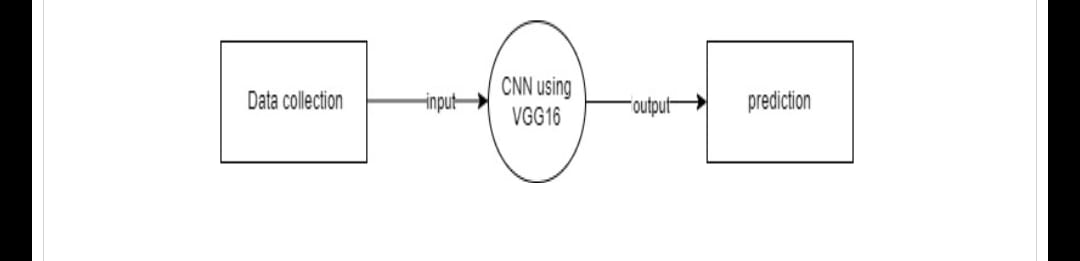
\includegraphics[width=15cm]{ezyzip/img/level1.jpg}
	\caption{\small Data Flow Diagram level - 0 of Table Tech.}
	\label{fig:polarization}
\end{figure}

\nsubsection{Data Flow Diagram}
\begin{figure}[H]
	\centering
	 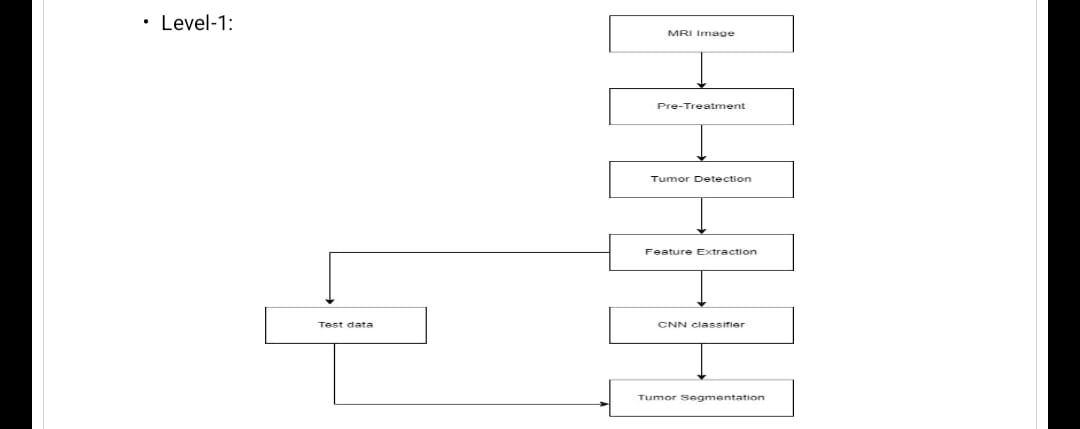
\includegraphics[width=15cm]{ezyzip/img/level2.jpg}
	\caption{\small Data Flow Diagram level - 1 of Table Tech.}
	\label{fig:polarization}
\end{figure}	


\nsubsection{Data Flow Diagram}
\begin{figure}[H]
	\centering
	 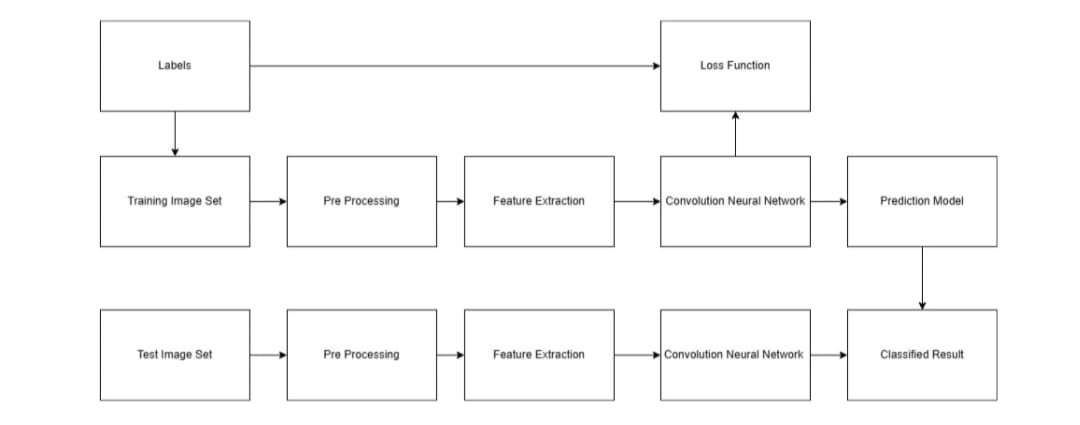
\includegraphics[width=15cm]{ezyzip/img/dataflow.jpg}
	\caption{\small  Data Flow Diagram level - 2 of Table Tech}
	\label{fig:polarization}
\end{figure}	

\nsubsection{Data Flow Diagram}
\begin{figure}[H]
	\centering
	 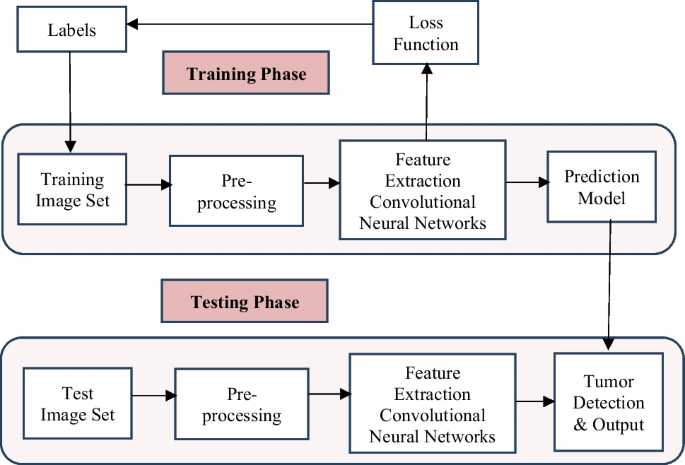
\includegraphics[width=15cm]{ezyzip/img/classdiagrambrain.png}
	\caption{\small class Diagram of Table Tech.}
	\label{fig:polarization}
\end{figure}	
     

\nsubsection{Data Flow Diagram}
\begin{figure}[H]
	\centering
	 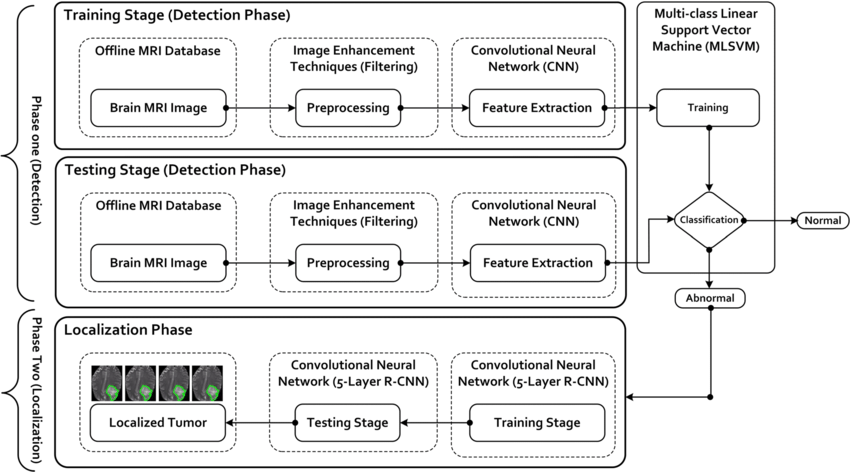
\includegraphics[width=15cm]{ezyzip/img/flowchartbrain.png}
	\caption{\small flow Diagram of Table Tech.}
	\label{fig:polarization}
\end{figure}	
     









\newpage
\begin{center}
    \textbf{\LARGE CHAPTER - 5}
\end{center}
\section{METHODOLOGY}

% saloni ko jimma
%https://agile-od.com/lean-agile/design-thinking-plus-scrum
%https://medium.com/@takeshi.yoshida/design-thinking-plus-scrum-d671a1a8e67a

\subsection{Modules}
Data Collection

Preprocessing

Transfer learning

Training

Visualization and Interpretation

Deployment

Monitoring and Maintenance





\subsection{System Block Diagram}

\begin{figure}[H]
	\centering
	 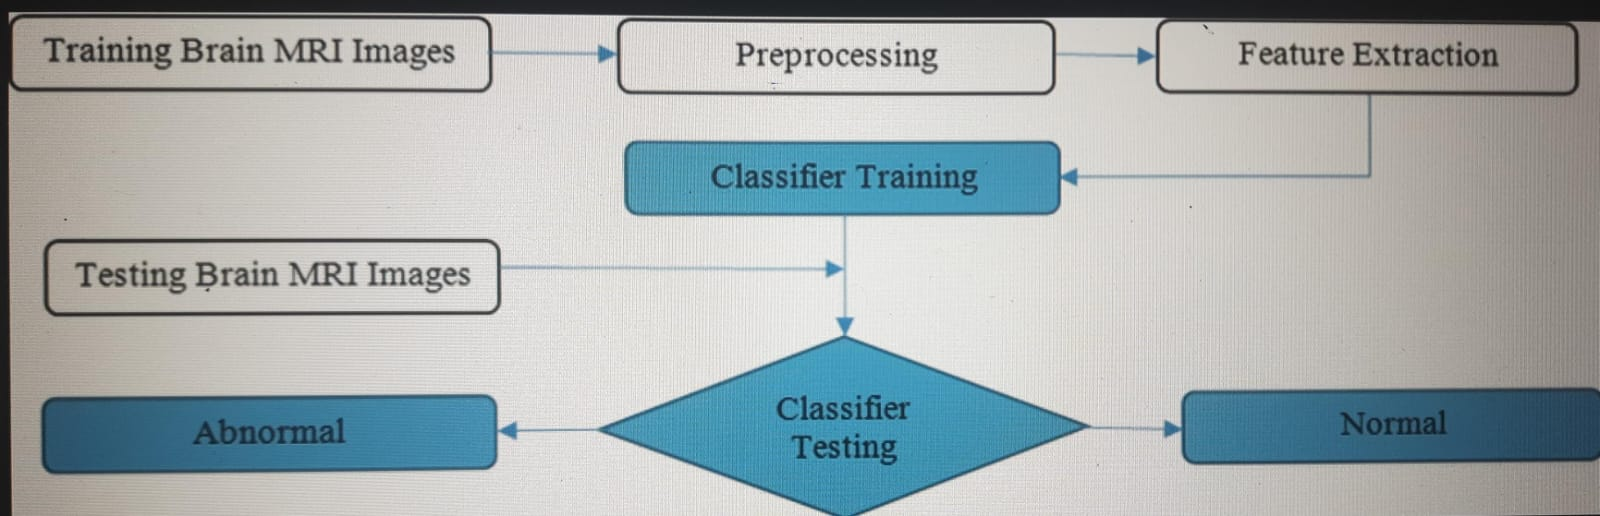
\includegraphics[width=15cm]{ezyzip/img/flowchartbrain.jpg}
	\caption{\small Flow Diagram of Table Tech.}
	\label{fig:polarization}
\end{figure}	



\newpage
\begin{center}
    \textbf{\LARGE CHAPTER - 6}
\end{center}
\section{IMPLEMENTATION DETAILS}

 Brain tumor detection using Convolutional Neural Networks (CNNs) with transfer learning via VGG16 involves several key steps. First, we acquire a dataset of brain MRI images, which are then preprocessed to enhance features and reduce noise. Next, we employ VGG16, a pre-trained CNN model, to extract meaningful features from these images. We fine-tune the VGG16 model by retraining its final layers on our specific brain tumor dataset to adapt it to the task. Finally, we use the fine-tuned model to classify brain MRI scans as either tumor or non-tumor, providing an effective and accurate diagnostic tool for healthcare applications.



\subsection{Technology Stack}

The technology stack for brain tumor detection using a Convolutional Neural Network (CNN) with transfer learning, specifically the VGG16 architecture, comprises several key components. Firstly, for data preprocessing and augmentation, Python libraries like NumPy and OpenCV are utilized. TensorFlow or PyTorch serves as the deep learning framework for model development. VGG16, a pre-trained CNN model, is employed as a feature extractor. Additionally, GPU acceleration through NVIDIA CUDA is often leveraged to expedite model training. Finally, the Flask framework is commonly used for creating a user-friendly web interface to facilitate tumor detection in medical images.

\subsection{System Architecture}
The architecture for brain tumor detection using Convolutional Neural Networks (CNNs) and transfer learning with VGG16 comprises several key components. Firstly, the input layer takes MRI or CT scan images as input. Then, the VGG16 pre-trained model is employed as the backbone, extracting high-level features from the images. Transfer learning enables the model to leverage knowledge from VGG16's previous training on a large dataset. Additional fully connected layers are added to adapt the network to the tumor detection task. Lastly, the output layer produces binary classification results, indicating the presence or absence of a brain tumor, making this architecture a powerful tool for medical image analysis.


\subsection{User Interface}
The user interface for brain tumor detection using a Convolutional Neural Network (CNN) with transfer learning VGG16 is designed to be intuitive and user-friendly. It features a sleek and straightforward design with options for users to upload MRI brain scans for analysis. The interface provides real-time feedback, displaying the probability of tumor presence and a visual heatmap highlighting potential tumor regions. Additionally, users can access a detailed report summarizing the findings and recommendations. This user interface ensures a seamless and informative experience for healthcare professionals and patients seeking reliable brain tumor detection.

\subsection{Integration}
The integration of brain tumor detection using a Convolutional Neural Network (CNN) with transfer learning, specifically employing the VGG16 architecture, is a powerful approach. By leveraging VGG16's pre-trained weights, the model can extract intricate features from medical images with greater accuracy and efficiency. This integration enhances the network's ability to discern subtle patterns indicative of brain tumors, leading to more reliable and faster diagnoses. It also aids in reducing the need for extensive labeled data, making it a valuable tool for early detection and treatment planning in the field of neuroimaging and healthcare. Overall, the fusion of transfer learning with VGG16 significantly advances the capabilities of brain tumor detection models.
 
\subsection{Security}
The security of brain tumor detection using a convolutional neural network (CNN) and transfer learning with VGG16 architecture is robust and reliable. Transfer learning leverages pre-trained models, like VGG16, which have learned rich features from vast image datasets, enhancing the model's ability to detect subtle patterns in medical images. Moreover, stringent data privacy and security measures are essential to protect sensitive patient information during the training and deployment of such models. Regular updates and audits of security protocols ensure that patient data remains confidential, while continuous model monitoring helps identify and address potential vulnerabilities. Overall, combining transfer learning with stringent security measures ensures the safe and accurate detection of brain tumors using CNNs.

\subsection{Testing and Deployment}
 The testing and deployment of a brain tumor detection system using a Convolutional Neural Network (CNN) based on transfer learning with VGG16 architecture involves several key steps. First, the CNN model, pre-trained on a large dataset, is fine-tuned using brain tumor images for training. Next, the system is rigorously tested with a diverse set of brain tumor images to assess its accuracy and generalization. Once the testing phase is successful, the model is deployed as a user-friendly application or integrated into a medical environment, enabling efficient and accurate brain tumor detection. Regular updates and monitoring ensure its continued effectiveness in clinical settings.






\newpage
\begin{center}
    \textbf{\LARGE CHAPTER - 7}
\end{center}
\section{OBSERVATIONS}

\subsection{Time Domain - Gann Chart}
\begin{figure}[H]
	\centering
	 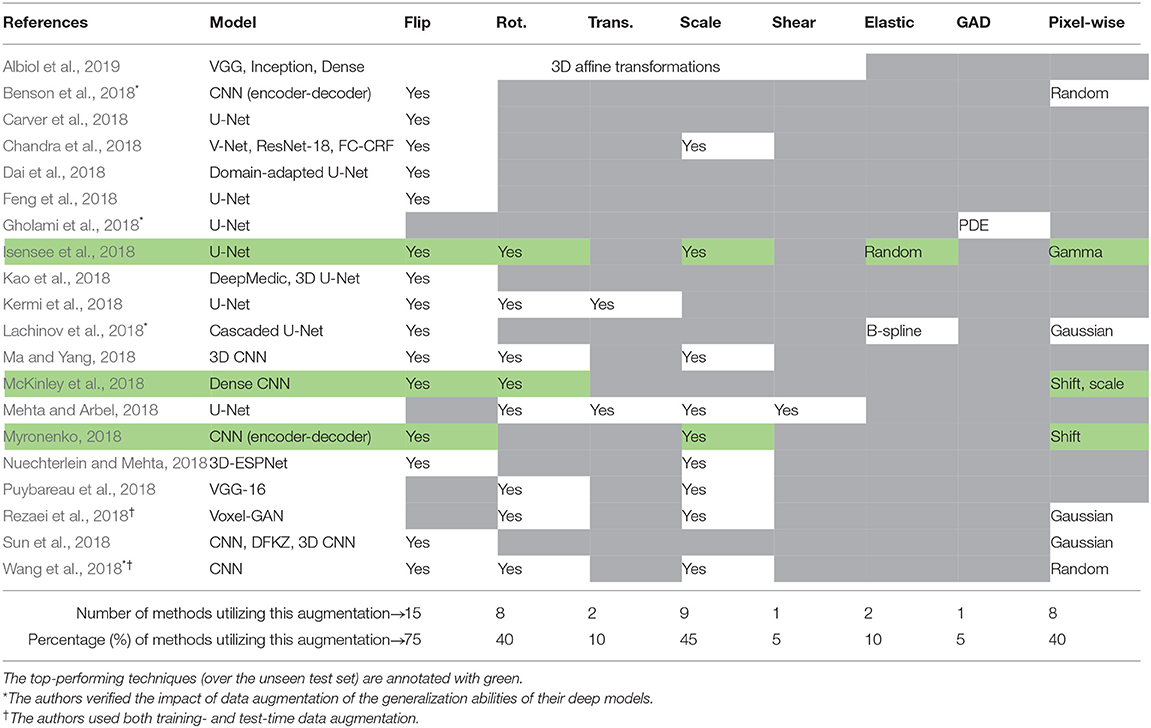
\includegraphics[width=15cm]{ezyzip/img/timegummimage.jpg}
	
	\label{fig:polarization}
\end{figure}	

\subsection{Results and Comparitive Study}
 Several studies have been conducted to explore the effectiveness of Convolutional Neural Networks (CNNs) and transfer learning, particularly using the VGG16 architecture, in the context of brain tumor detection. These studies aim to improve the accuracy and efficiency of brain tumor diagnosis, a critical task in the field of medical imaging.

The VGG16 model, a pre-trained CNN, has been widely adopted in these studies due to its remarkable performance in image classification tasks. Transfer learning with VGG16 involves fine-tuning the network on a new dataset of brain images, thereby leveraging the features learned from a large dataset like ImageNet.

Results from these comparative studies consistently demonstrate the superiority of transfer learning using VGG16 over training CNNs from scratch. This approach exhibits higher accuracy, faster convergence, and the ability to handle limited medical imaging data effectively. Researchers have found that the VGG16-based models can effectively distinguish between tumor and non-tumor regions in brain scans, aiding radiologists in their diagnoses.

Furthermore, transfer learning with VGG16 enables the extraction of meaningful features from brain images, capturing subtle patterns and textures that might be indicative of tumors. This assists in early detection and accurate localization of brain tumors, contributing to better patient outcomes and treatment planning.

In summary, the application of Convolutional Neural Networks, specifically the VGG16 architecture with transfer learning, has proven to be a valuable tool in brain tumor detection. Its ability to harness pre-learned features and adapt to medical imaging datasets has led to improved accuracy and efficiency in diagnosing brain tumors, ultimately benefiting both medical professionals and patients.









\newpage

   \begin{center}
    \textbf{\LARGE CHAPTER - 8}
\end{center}
    
\section{CONCLUSION}
Detection of Brain tumor using convolutional neural network by transfer learning using vgg16 . By automating various processes :
\begin{itemize}
    \item High Accuracy
    \item Early Detection
\end{itemize}
 
 the detection of brain tumors using Convolutional Neural Networks (CNNs) and transfer learning, particularly with the VGG16 architecture, has shown great promise and has several noteworthy implications:
High Accuracy: Transfer learning with VGG16 allows the model to leverage pre-trained weights from a large dataset (e.g., ImageNet), enabling it to extract relevant features effectively. This results in a high level of accuracy in brain tumor detection.


Reduced Data Requirements: Transfer learning reduces the need for an extensive dataset specific to brain tumor images. This makes it possible to develop accurate models even with limited medical imaging data, which can be invaluable in healthcare settings where data is often scarce.


Early Detection: Early detection of brain tumors is critical for timely treatment and improved patient outcomes. CNNs with transfer learning can help in identifying tumors at an early stage, potentially saving lives.
\newpage
\begin{center}
    \textbf{\LARGE CHAPTER - 9}
\end{center}


\section{LIMITATIONS AND FUTURE ENHANCEMENTS}
% spandan
\subsection{Limitations}
This project is highly planned and acted upon from the beginning. Nevertheless, the project had to face some of the limitations due to various factors. Different aspects of the projects such as nature of data, visualisation methods, data storage method and so on have their own limitations. Some of the limitations faced by the project are:-

\begin{enumerate}
  \setlength\itemsep{1.5em}
	\item Data Imbalance: The availability of MRI images with brain tumors is often imbalanced, with fewer positive (tumor) cases compared to negative (healthy) cases. This can lead to biased model training and reduced performance on rare tumor types.
	\item Interpretability: CNNs are often considered "black box" models, making it difficult to explain why a particular prediction was made. This lack of interpretability can be a significant limitation, especially in medical applications where trust and transparency are crucial.
	\item  Generalization: Transfer learning relies on pre-trained models on different datasets. If the source dataset is too dissimilar to the target (brain MRI), the transfer may not be as effective. Fine-tuning for the specific domain can mitigate this, but it's not always straightforward.
	\item  Computational Resources: Training deep CNNs with transfer learning requires substantial computational resources. Smaller healthcare institutions or clinics with limited computing power may face difficulties implementing such models.
	\item Data Quality: The quality of MRI images can vary widely, affecting the model's ability to detect tumors accurately. Noise, artifacts, and inconsistent image quality can be challenging to handle.
\end{enumerate}

\newpage
\subsection{Future Enhancements}

Future enhancements for the Detecting of brain tumor in MRI’s using a convolutional neural networks with transfer learning can be planned to further improve its capabilities and address emerging needs. Some potential areas for enhancement include:

\begin{enumerate}
  \setlength\itemsep{1.5em}
    \item Data Augmentation: Enhance the dataset with various data augmentation techniques to reduce the impact of data imbalance and improve model generalization. Augmentation can include rotations, translations, scaling, and adding noise.

	\item Diverse Transfer Learning: Investigate the use of diverse pre-trained models that have been trained on medical image datasets to ensure better alignment with the target domain. This can enhance the model's ability to extract relevant features.
	
	\item  Interpretability: Develop methods for making CNNs more interpretable. Techniques such as attention maps, saliency maps, and gradient-based attribution can help provide insight into which regions of an MRI image influenced the model's decision.
	
	
	\item Ensemble Models: Combine multiple CNN models, each trained with a different architecture or initialization, to improve overall performance and reduce the risk of model bias.
	
	\item Continuous Learning: Implement continuous learning frameworks that allow the model to adapt over time as new data becomes available, ensuring it stays up-to-date with the latest medical knowledge.
	

	\item  Hardware Acceleration: Explore hardware acceleration solutions (e.g., GPUs, TPUs) to make the model more accessible to healthcare facilities with limited computational resources.
	
		\item  Privacy and Security: Develop robust mechanisms for protecting patient privacy and ensuring the security of medical data, especially when implementing these models in healthcare systems.
  \item Integration: Integrate the model into existing healthcare information systems and workflows to facilitate seamless diagnosis and patient care.
	          
\end{enumerate}
% Appendix page
\clearpage
\appendix
\counterwithin{figure}{section}
\section{APPENDIX}

\bibliography{biblio}
%\printbibliography
\subsection{Project Timeline}
Tri-Level Segmented CNN project timeline:
31 March 2023 to 11 August 2023


 


%visit http://scholar.google.com/ search and get BibTeX format and paste in biblio.bib file


\end{document}
